\section{Frontend}\label{sec:poc:frontend}
Das Frontent ist in \acl{js} und \acs{html}, mit VueX als Framework geschrieben.

\begin{figure}[ht]
  \centering
  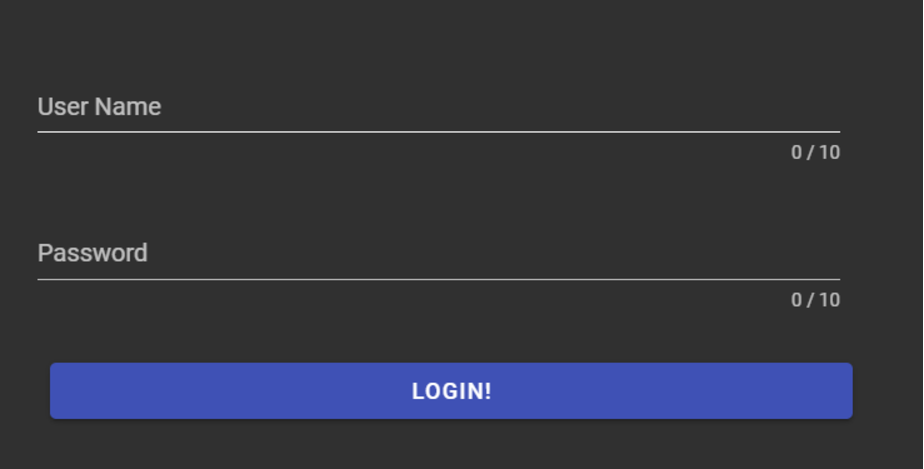
\includegraphics[width=\textwidth]{content/hauptteil/umsetzungPoC/frontend/res/screenLogin.pdf}
  \caption{Screenshot der Login Seite}
  \label{fig:frontend:poc:login}
\end{figure}


\begin{figure}[ht]
  \centering
  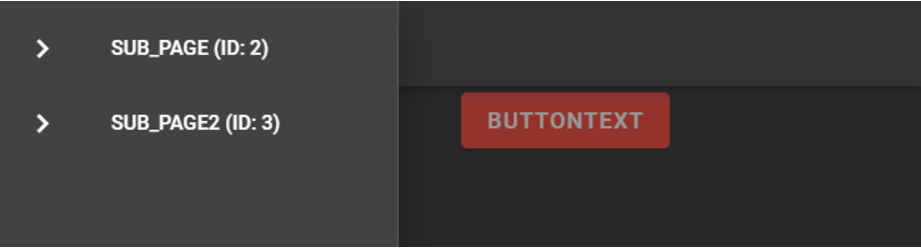
\includegraphics[width=\textwidth]{content/hauptteil/umsetzungPoC/frontend/res/screenPageNav.pdf}
  \caption{Screenshot einer Beispielseite mit ausgeklappter Navigation}
  \label{fig:frontend:poc:nav}
\end{figure}


\begin{figure}[ht]
  \centering
  \begin{subfigure}[b]{\textwidth}
    \centering
    
\includegraphics[width=\textwidth]{content/hauptteil/umsetzungPoC/frontend/res/screenPage.pdf}
    \caption{\emph{DataNode} \eigenName{ButtonState} = \emph{false}}
    \label{fig:frontend:poc:button:true}
  \end{subfigure}
  \hspace{50.00mm}
  \begin{subfigure}[b]{\textwidth}
      \centering
      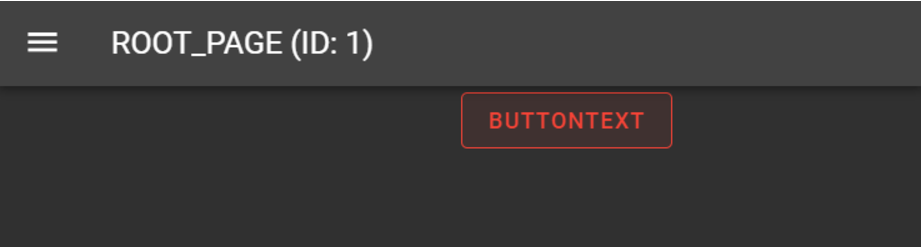
\includegraphics[width=\textwidth]{content/hauptteil/umsetzungPoC/frontend/res/screenButtonClicked.pdf}
      \caption{\emph{DataNode} \eigenName{ButtonState} = \emph{false}}
      \label{fig:frontend:poc:button:false}
  \end{subfigure}
  \caption[Screenshot einer Seite mit Button]{Screenshot einer Seite mit Button in zwei verschiedenen Zuständen}
  \label{fig:frontend:poc:button}
\end{figure}

